\documentclass[10pt]{beamer}

\mode<presentation>{% Settings
    % link to view http://www.hartwork.org/beamer-theme-matrix/
    % ------------------------------------------------------------------------------
    % Slide Themes
    % ------------------------------------------------------------------------------
    %\usetheme{default}
    %\usetheme{AnnArbor}
    %\usetheme{Antibes}
    %\usetheme{Bergen}
    \usetheme{Berkeley}
    %\usetheme{Berlin}
    %\usetheme{Boadilla}
    %\usetheme{CambridgeUS}
    %\usetheme{Copenhagen}
    %\usetheme{Darmstadt}
    %\usetheme{Dresden}
    %\usetheme{Frankfurt}
    %\usetheme{Goettingen}
    %\usetheme{Hannover}
    %\usetheme{Ilmenau}
    %\usetheme{JuanLesPins} % rounded title, gradient at top with section, no bottom bar
    %\usetheme{Luebeck}     % square title, toc at top of each slide 
    %\usetheme{Madrid}      % rounded title
    %\usetheme{Malmoe}
    %\usetheme{Marburg}
    %\usetheme{Montpellier}
    %\usetheme{PaloAlto}
    %\usetheme{Pittsburgh}
    %\usetheme{Rochester}
    %\usetheme{Singapore}
    %\usetheme{Szeged}
    %\usetheme{Warsaw}

    % ------------------------------------------------------------------------------
    % Color Schemes
    % ------------------------------------------------------------------------------
    %\usecolortheme{default}
    %\usecolortheme{albatross}  % blue background with darker blue
    %\usecolortheme{beaver}     % gray with red
    %\usecolortheme{beetle}     % gray background
    %\usecolortheme{crane}      % orange
    \usecolortheme{dolphin}     % white with purple
    %\usecolortheme{dove}       % all white
    %\usecolortheme{fly}        % all gray including background
    %\usecolortheme{lily}       % white with blue
    %\usecolortheme{orchid}     % default blue
    %\usecolortheme{rose}       % default blue
    %\usecolortheme{seagull}    % darker gray than seahorse
    %\usecolortheme{seahorse}   % light gray blueish tint
    %\usecolortheme{whale}      % default blue
    %\usecolortheme{wolverine}  % yellow with a little blue

    %\setbeamertemplate{footline} % To remove the footer line in all slides uncomment this line
    %\setbeamertemplate{footline}[page number] % To replace the footer line in all slides with a simple slide count uncomment this line
    \setbeamertemplate{navigation symbols}{} % To remove the navigation symbols from the bottom of all slides uncomment this line
    \setbeamertemplate{bibliography item}{\insertbiblabel} % to number bibliography entries
}

\usepackage{Logemann}
\usepackage{Integral}
\usepackage{Derivative}
\usepackage{Sum}
\usepackage[backend=biber]{biblatex}
\addbibresource{refs.bib}

\title[]{Discontinuous Galerkin Method for solving a Thin-Film Equation} % The short title
% appears at the bottom of every slide, the full title is only on the title page

\author{Caleb Logemann} % Your name
\institute[Iowa State University]{% Your institution as it will appear on the bottom of every slide, may be shorthand to save space
Mathematics Department, Iowa State University \\ % Your institution for the title page
\medskip
\textit{logemann@iastate.edu}} % Your email address

\date{September 30, 2017} % Date, can be changed to a custom date

\begin{document}
  \begin{frame}
    \titlepage{}
  \end{frame}

  \begin{frame}
    \frametitle{Overview}
    \tableofcontents
  \end{frame}

  \section{Introduction}
    \begin{frame}
      \frametitle{Motivation}
      \begin{itemize}
        \item Aircraft Icing
        \item Runback
      \end{itemize}
      \begin{center}
        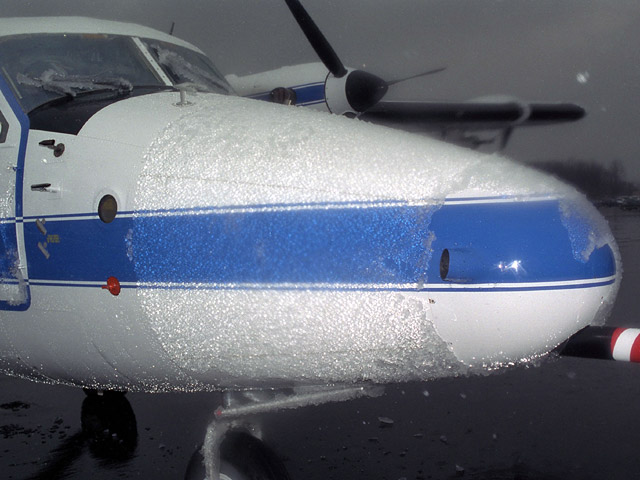
\includegraphics[scale=0.2]{Figures/Icing_on_a_plane.jpg}
        \hspace{0.1in}
        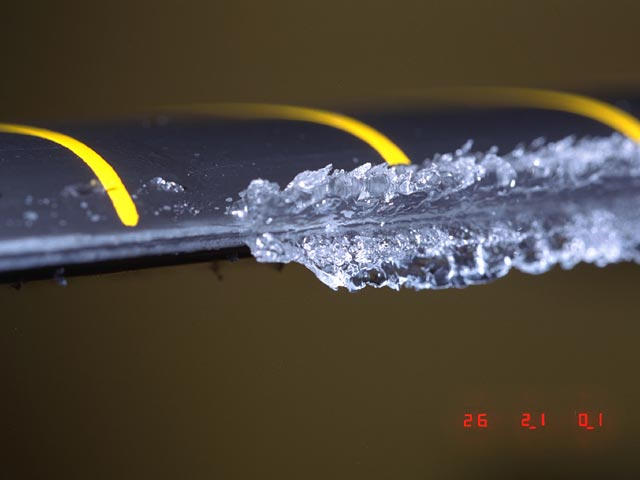
\includegraphics[scale=0.2]{Figures/Icing_on_a_rotor.jpg}
      \end{center}
      \begin{itemize}
        \item Industrial Coating
        \item Paint Drying
      \end{itemize}
    \end{frame}

    \begin{frame}
      \frametitle{Model Equations}
      \begin{itemize}
        \item Navier-Stokes Equation
          \begin{align*}
            \rho_t + \p{\rho u}_x &= 0 \\
            \p{\rho u}_t + \p{\rho u^2 + p}_x &=  \\
            E_t + \p{u (E + p)}_x &= \\
          \end{align*}

        \item Asymptotic Limit, $\rho << L$
        \item Thin-Film Equation - 1D with $u$ as fluid height.
          \[
            u_t + \p{f(x, t) u^2 - g(x, t) u^3}_x = \p{h(x, t) u^3 u_{xxx}}_x
          \]
      \end{itemize}
    \end{frame}

    \begin{frame}
      \frametitle{Current Model}
      \begin{itemize}
        \item Simplified Expression
          \[
            u_t + \p{u^2 - u^3}_x = \p{u^3 u_{xxx}}_x
          \]

        \item Operator Splitting
          \begin{align*}
            u_t + \p{u^2 - u^3}_x &= 0 \\
            u_t - \p{u^3 u_{xxx}}_x &= 0
          \end{align*}
      \end{itemize}
    \end{frame}

    \begin{frame}
      \frametitle{Introduction to Discontinuous Galerkin}
      \begin{itemize}
        \item Partition the domain, $\br{a, b}$ as
          \[
            a = x_{1/2} < \cdots < x_{i-1/2} < x_{i+1/2} < \cdots < x_{N + 1/2} = b
          \]

        \item $V_i = \br{x_{i-1/2}, x_{i+1/2}}$
        \item $\Delta x = x_{i + 1/2} - x_{i - 1/2}$
        \item $x_i = \frac{x_{i+1/2} + x_{i-1/2}}{2}$.
          \begin{center}
            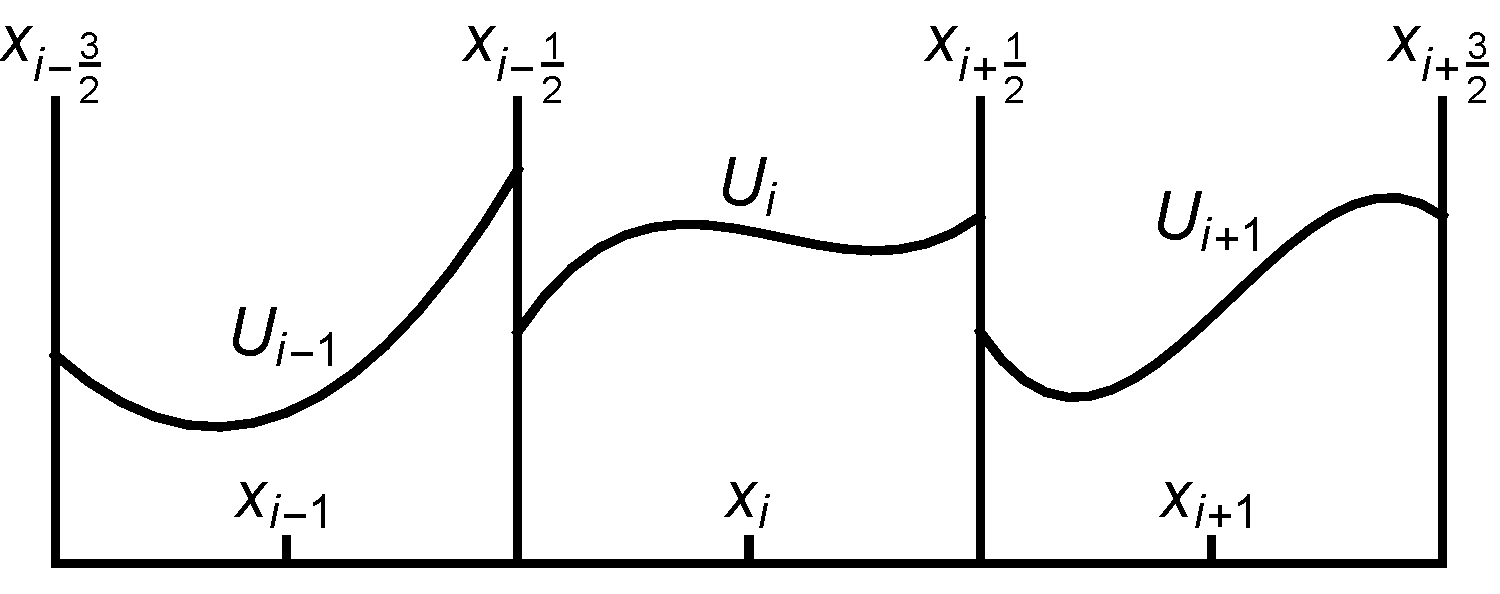
\includegraphics[scale=0.2]{Figures/DG.pdf}
          \end{center}

        \item Solution of order $M$ on each cell
          \[
            \eval{u}{x \in V_i}{} \approx U_i = \sum*{k = 1}{M}{U_i^k \phi^k(\xi)}
          \]

        \item Legendre Basis - $\phi^k$
      \end{itemize}
    \end{frame}

    \begin{frame}
      \frametitle{Numerical Solutions}
      \begin{itemize}
        \item Use canonical variable $\xi \in \br{-1, 1}$
        \item Let $\set{\phi^k(\xi)}$ be the Legendre polynomials.

        \item Solution of order $M$ on each cell
          \[
            \eval{u}{x \in V_i}{} \approx U_i = \sum*{k = 1}{M}{U_i^k \phi^k(\xi)}
          \]
      \end{itemize}
    \end{frame}

  \section{Convection}
    \begin{frame}
      \frametitle{Convection}
      \begin{itemize}
        \item Convection Equation
          \[
            u_t + \p{u^2 - u^3}_x = 0
          \]

        \item Weak Form
          \[
            \dintt{-1}{1}{u_t \phi(\xi) + \frac{2}{\Delta x}\p{u^2 - u^3}_\xi \phi}{\xi}
          \]

        \item Runge-Kutta Discontinuous Galerkin


      \end{itemize}
    \end{frame}

    \begin{frame}
      \frametitle{Numerical Example - Square Wave}
      \begin{center}
        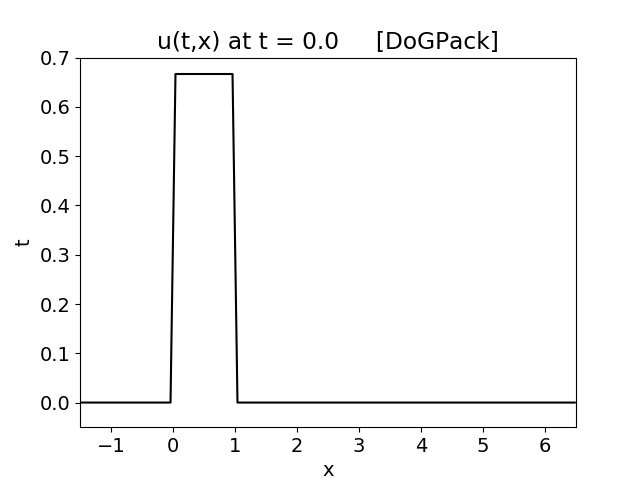
\includegraphics[scale=0.6]{Figures/squarewave00.png}
      \end{center}
    \end{frame}
    \begin{frame}
      \frametitle{Numerical Example - Square Wave}
      \begin{center}
        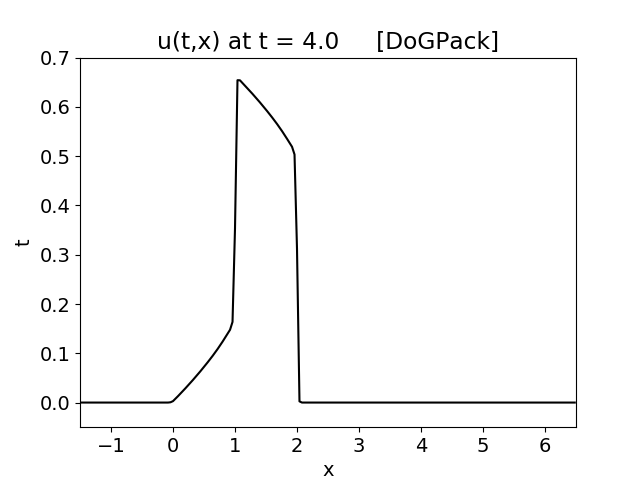
\includegraphics[scale=0.5]{Figures/squarewave04.png}
      \end{center}
    \end{frame}
    \begin{frame}
      \frametitle{Numerical Example - Square Wave}
      \begin{center}
        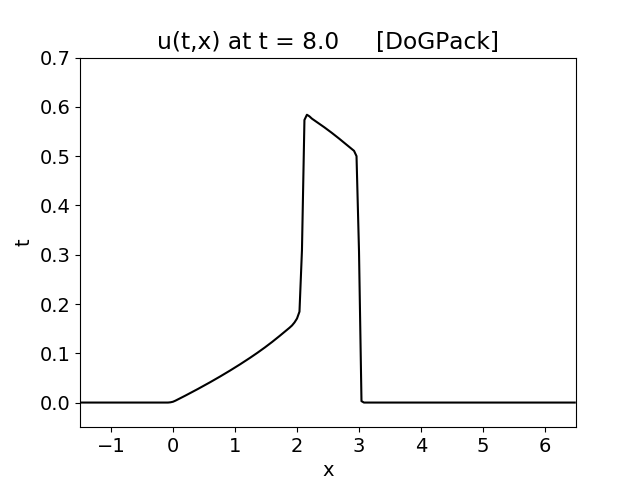
\includegraphics[scale=0.6]{Figures/squarewave08.png}
      \end{center}
    \end{frame}
    \begin{frame}
      \frametitle{Numerical Example - Square Wave}
      \begin{center}
        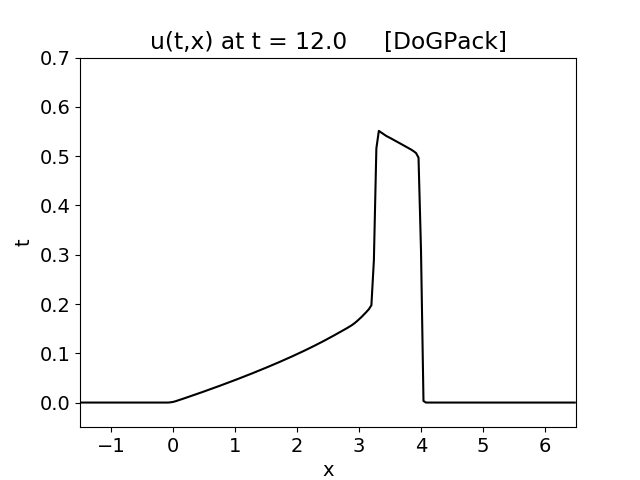
\includegraphics[scale=0.6]{Figures/squarewave12.png}
      \end{center}
    \end{frame}
    \begin{frame}
      \frametitle{Numerical Example - Square Wave}
      \begin{center}
        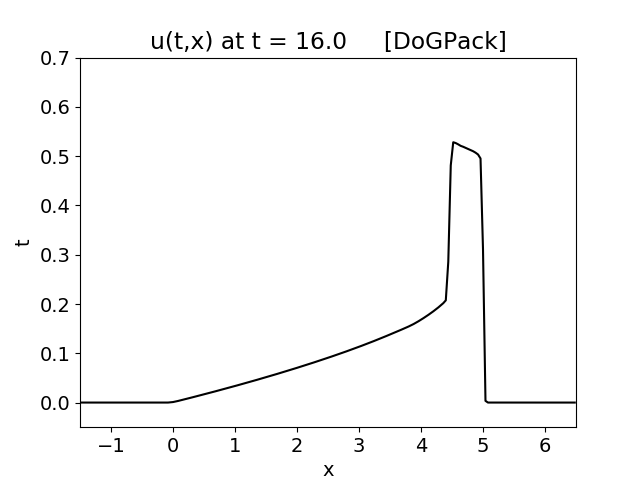
\includegraphics[scale=0.6]{Figures/squarewave16.png}
      \end{center}
    \end{frame}
    \begin{frame}
      \frametitle{Numerical Example - Square Wave}
      \begin{center}
        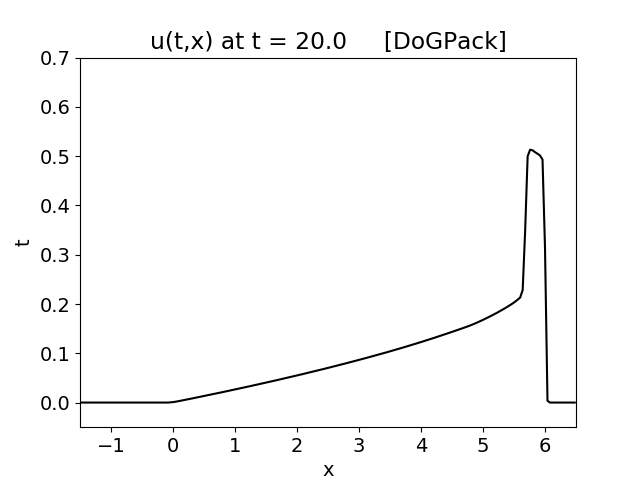
\includegraphics[scale=0.6]{Figures/squarewave20.png}
      \end{center}
    \end{frame}

  \section{Diffusion}
    \begin{frame}
      \frametitle{Diffusion}
      \begin{itemize}
        \item Diffusion Equation
          \[
            u_t - \p{u^3 u_{xxx}}_x = 0
          \]

        \item Local Discontinuous Galerkin

      \end{itemize}
    \end{frame}

    \begin{frame}
      \frametitle{Multigrid Solver}

    \end{frame}

    \begin{frame}
      \frametitle{Numerical Results}

    \end{frame}

  \section{Conclusion}
    \begin{frame}
      \frametitle{Future Work}
      \begin{itemize}
        \item Higher dimensions
        \item Curved surfaces
        \item Space and time dependent coefficients
        \item Incorporation with air flow models
      \end{itemize}
    \end{frame}

    \begin{frame}
      \frametitle{Conclusion}
      \begin{itemize}
        \item Questions?
      \end{itemize}
    \end{frame}

    \begin{frame}
      \frametitle{Bibliography}
      % TODO: Bibliography
      \nocite{*}
      \printbibliography{}
    \end{frame}
\end{document}
